\documentclass[11pt, a4paper]{article}

\usepackage{ctex}
\usepackage{geometry}
\usepackage{amsmath}
\usepackage{amssymb}

\geometry{bottom=2cm, top=2cm, left=1.5cm, right=1.5cm}

\begin{document}
	
\title{微分方程实验一:线性有限元方法求解两点边值问题}
\author{15336134 莫凡}
\maketitle

\section{实验假设}

使用线性有限元方法求解两点边值问题
\begin{equation}
\begin{array}{c}
Lu=-\dfrac{\mathrm{d}}{\mathrm{d}x}\left(p\dfrac{\mathrm{d}u}{\mathrm{d}x}\right)+qu=f\quad x\in (a, b)\\
u(a)=0,u'(b)=0
\end{array}
\end{equation}

将问题具体化,假设问题为书后P47中的
\begin{equation}
p=1,~q=\dfrac{\pi^2}{4},~f=\dfrac{\pi^2}{2}\sin\dfrac{\pi}{2}x,~a=0,~b=0
\end{equation}

\section{实验过程}
首先按照高斯分布随机一组$(0,1)$中的向量,排序去重之后得到$x$

然后预处理出两点间隔距离向量$h$,$Q_i=h_i^{-1}p(x_{i-1}+yh_i\xi)$以及$\xi_i=\dfrac{x-x_{i-1}}{h_i}$

构建单元刚度矩阵
\begin{equation}
K^{(i)}=
\begin{pmatrix}
\int_{0}^{1}[Q_i+h_iq(x_{i-1}+h_i\xi)(1-\xi)^2]\mathrm{d}\xi &
\int_{0}^{1}[-Q_i+h_iq(x_{i-1}+h_i\xi)\xi(1-\xi)]\mathrm{d}\xi \\
\int_{0}^{1}[-Q_i+h_iq(x_{i-1}+h_i\xi)\xi(1-\xi)]\mathrm{d}\xi &
\int_{0}^{1}[Q_i+h_iq(x_{i-1}+h_i\xi)\xi^2]\mathrm{d}\xi 
\end{pmatrix}
\end{equation}

然后求和得到一个刚度矩阵
\begin{equation}
K=\sum_{i=1}^nK^{(i)}
\end{equation}

接下来令
\begin{equation}
\left\{
\begin{array}{l}
f_{i-1}^{(i)}=h_i\int_0^1f(x_{i-1}+h_i\xi)(1-\xi)\mathrm{d}\xi\\
f_{i}^{(i)}=h_i\int_0^1f(x_{i-1}+h_i\xi)\xi\mathrm{d}\xi
\end{array}
\right.
\end{equation}

\begin{equation}
b_i=f_i^{(i)}+f_i^{(i+1)},b_n=f_n^{(n)}
\end{equation}

求解线性方程组
\begin{equation}
Ku=b
\end{equation}

在具体实现中数值积分使用辛普森公式,线性方程组使用直接解法。由于K是大型对角矩阵,后期将改用高斯塞德尔迭代求解。目前$n$的规模限制在100以内,所以影响不大。具体见代码文件,不在此处粘贴代码

\section{实验结果}

得到的是一个近似的分段线性函数。采用画图的方法将其表示出来

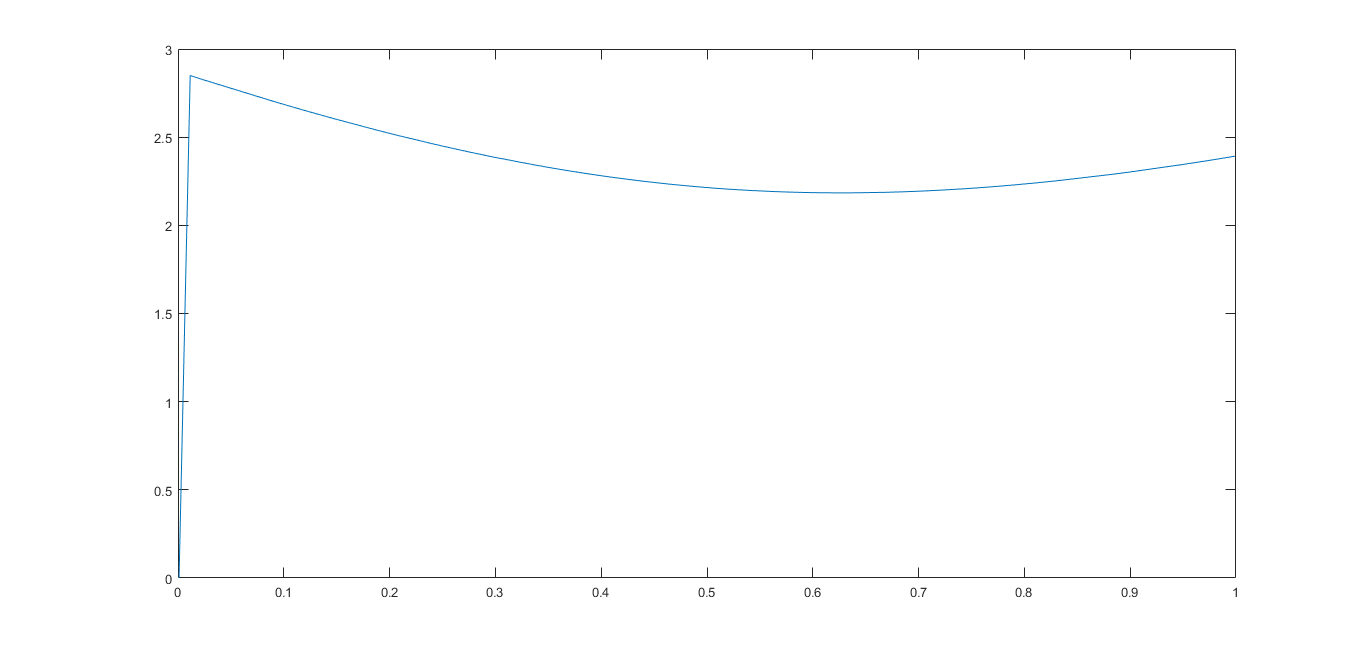
\includegraphics[width=400pt]{result.png}

除去左边的部分是由插值点的选取(高斯分布)、数值方法的误差导致,其余部分是一个近似光滑的函数,对比原函数解析解,基本合乎要求

\section{附件}
\begin{itemize}
	\item linear\_element.m 线性有限元方法程序
	\item script.m 运行主程序
\end{itemize}
\end{document}